\chapter{文獻回顧}
\fontsize{12pt}{18pt}\selectfont %字體大小,行距

% ------------------------- 2.0 ------------------------- %
本論文研究主題為探討如何利用 IMU 提升人體姿態量測、估計與重建的成功率,並降低其使用門檻。因此,本章節將針對人體姿態估計的相關文獻進行回顧與討論,內容包括動作捕捉系統及相關感測器的應用、人體模型種類、時間同步方法、感測器融合演算法等,統整現今常見技術,並說明其原理、特色、目前可達到的精度、優缺點等,以作為本研究之基礎。

% ------------------------- 2.1 ------------------------- %
\section{動作捕捉系統}
% 概述人體動作捕捉,再說分為單感測器動作捕捉系統及多感測器動作捕捉系統,單感測動作捕捉系統又分為光學動作系統及無學動作捕捉系統
% 下面的子段落要寫的:原理、特色、目前可達到的誤差、優缺點
動作捕捉系統 (Motion Capture System) 為現今常用於擷取人體動作、表情、手勢或其他物體動作等資訊的技術,從而將人體姿態 (pose) 量化,其可應用於運動分析~\cite{armitano2022swot}、醫學研究~\cite{alarcon2020upper}~\cite{gu2023imu}、遊戲開發、影片製作等領域,藉由取得的資訊,可進行分析、模擬、辨識等應用。根據感測器種類及數量的不同,動作捕捉系統可分為單感測器動作捕捉系統及多感測器融合 (sensor fusion) 動作捕捉系統,其中單感測器動作捕捉系統又可分為光學動作捕捉系統及慣性動作捕捉系統。 

人體姿態 (pose) 可使用位置資訊 (position) 或朝向資訊 (orientation) 進行定義,位置資訊通常以笛卡爾坐標系 (Cartesian coordinate system) 描述物體在空間中的位置,因此可使用量測結果為位置資訊的光學動作捕捉系統 (optical motion capture, OMC) 進行姿態追蹤;而朝向資訊則常以尤拉角 (Euler angles) 、旋轉矩陣 (rotation matrix) 或四元數 (quaternions) 來描述物體的朝向狀態,因此可使用量測結果為朝向資訊的慣性動作捕捉系統 (inertial motion capture) 進行姿態追蹤。以下將針對光學動作捕捉系統、慣性動作捕捉系統、多感測器融合動作捕捉系統,這三大類系統進行介紹。

\subsection{單感測器-光學動作捕捉系統}
% 有沒有光標記的都放在這一段裡面一起描述,可能用句號分開就好
光學動作捕捉系統 (optical motion capture, OMC) 是目前最常見的動作捕捉系統,其原理為透過辨別標記點或特定特徵點的位置來追蹤物體的運動,再進一步由邊際點或特徵點的位置推估物體的姿態。根據受試者身上有無光標記 (marker),可將光學動作捕捉系統以有無光標記的分類方法細分為光標記捕捉系統 (marker-based motion capture) 及無標記捕捉系統 (markerless motion capture)。

\subsubsection{光標記動作捕捉系統}
% - 量測精確度高,作為目前開發其他動作捕捉系統的標準
% - 無法在室外量測
% - 器材架設不易,價格昂貴
% - 量測誤差約落在 1 公分
光標記動作捕捉系統 (marker-based motion capture),
如 Vicon ~\cite{vicon_web}是目前最常見且最精準的動作捕捉系統,
其在靜態實驗中,平均絕對定位誤差為 0.15 (mm)~\cite{merriaux2017study},
因此其量測結果常被當作正確答案,用於確認其他動作捕捉系統的準確性。
光標記動作捕捉系統所需量測設備為多個紅外光攝影機及多個反光標記點,
反光標記點需黏貼在受試者多處明顯不易被遮擋的部位,例如骨突點,確保在實驗過程中的多數時間可於影像中看見並被記錄,
而經過校正的多個紅外光攝影機需同時記錄下影像,確保不同角度間的影像無時間差,
每台紅外光攝影機可發出紅外光,也可接收反光標記點反射的紅外光,透過三角測量計算標記點的位置來推估受試者的姿態,
實驗環境及實驗設置如圖~\ref{ch2_fig_OMC_Vicon} 所示,可看到在右後方上側掛有紅外光攝影機,下方有一位穿著黑色緊身衣的受試者,經由量測可建立出圖中左下側螢幕中的人體姿態。
由於光標記動作捕捉系統主要傳遞訊息的媒介為紅外光,需要嚴格控管環境光(例如陽光)的影響,減少環境光造成的雜訊,
因此實驗環境多為使用人造光為主要照明的的室內,無法在會受到大量陽光干擾的室外進行量測,
且由於需使用多台攝影機,因此器材架設不易,價格昂貴。

\begin{figure}[!ht]
    \centering
    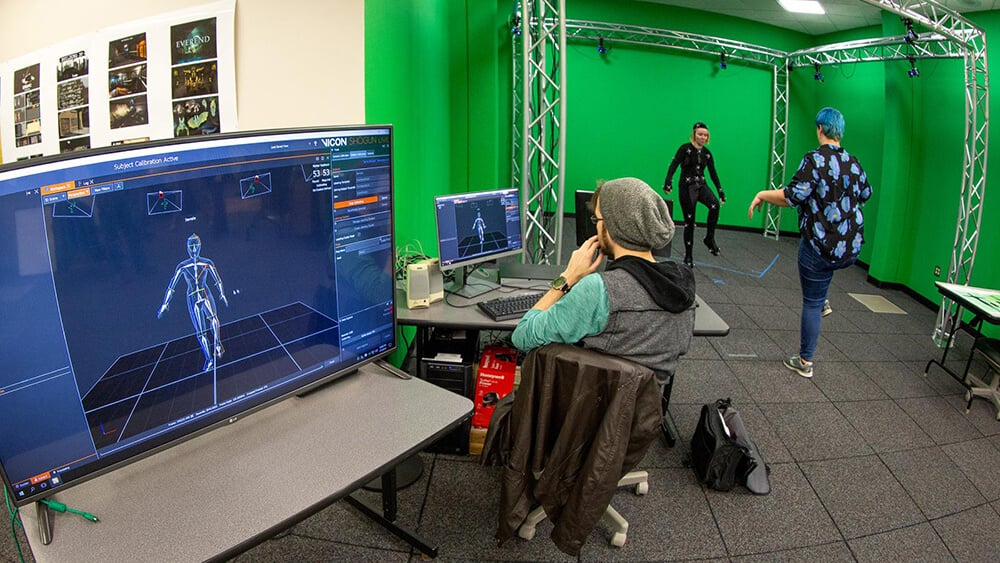
\includegraphics[width=8cm]{figure/ch2_fig_OMC_Vicon.jpg}
     \caption[Vicon 實驗環境與設置~\cite{vicon_web}]{Vicon 實驗環境與設置~\cite{vicon_web}}
     \label{ch2_fig_OMC_Vicon}
\end{figure}

\subsubsection{無標記動作捕捉系統}
% - OpenPose、MediaPipe
    % - 看一下 OpenPose 的文獻
    % - 可在室外量測
    % - 器材架設相對容易
    % - 量測誤差約落在 7.2 公分,精準程度會隨著相機數量的減少而降低
    % - 若被遮擋,則無法辨識出被遮擋的關節
    % - 上到下或下到上的辨識(不知道找不找得到相關有提到這方面的paper)
    % - 想想看要怎麼把兩種方法的辨識結果圖片塞進去
因為光標記動作捕捉系統的限制,加上電腦視覺與深度學習的崛起,無標記動作捕捉系統 (markerless motion capture) 逐漸受到重視~\cite{sarafianos20163d},
其中 OpenPose ~\cite{8765346}~\cite{wei2016cpm}~\cite{simon2017hand}~\cite{cao2017realtime}、
由 Google 團隊開發的 MediaPipe ~\cite{mediapipe_web} 及由 Microsoft 開發的 Kinect ~\cite{zhang2012microsoft} 等系統是目前常見的無標記動作捕捉系統,常被應用於偵測及重建人體姿態,或是估計關節角度~\cite{LATRECHE2023112826},
如圖~\ref{ch2_fig_rec_result} (a) 使用影像辨識方法偵測人體關節點,從而得出人體姿態,圖~\ref{ch2_fig_rec_result} (b) 則使用影像辨識方法先偵測出關節點,進而計算出關節角度。

\begin{figure}[!ht]
    \centering
    \begin{minipage}{.37\textwidth}
      \centering
      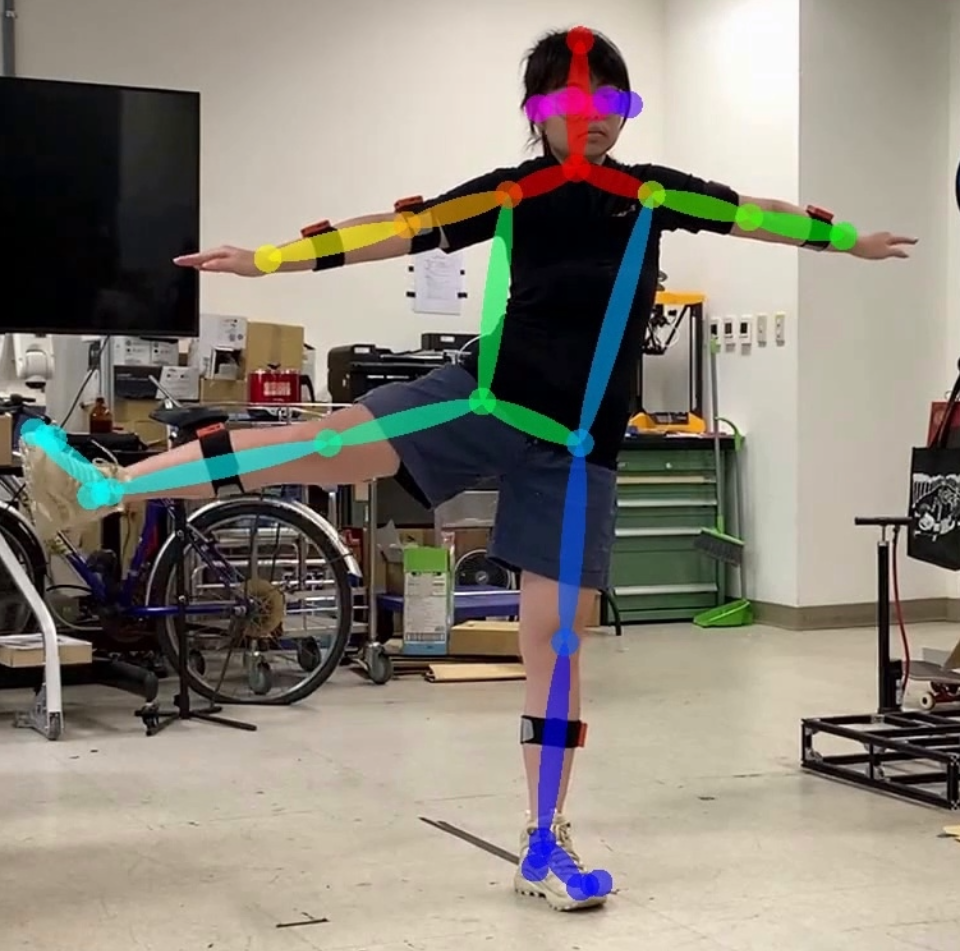
\includegraphics[width=.95\linewidth]{figure/ch2_fig_rec_openpose.png}
      \caption*{(a) 偵測人體姿態}
    \end{minipage}%
    \begin{minipage}{.63\textwidth}
       \centering
       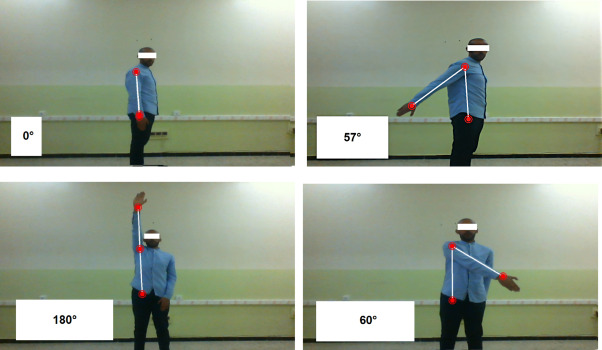
\includegraphics[width=.95\linewidth]{figure/ch2_fig_joint_angle.jpg}
       \caption*{(b) 估計關節角度~\cite{LATRECHE2023112826}}
    \end{minipage}
    \caption[無標記動作捕捉系統應用]{無標記動作捕捉系統應用}
    \label{ch2_fig_rec_result}
\end{figure}

透過已經過校正的單一或多個攝影機同時拍攝受試者的影像,利用電腦視覺及深度學習技術辨識出受試者在二維平面上的關節點位置,
辨識關節點位置的方法分為上到下方法 (top-down method) 及下到上方法 (bottom-up method) 兩種~\cite{nie2019single},
上到下方法如圖~\ref{ch2_fig_topvsbottom} 上半部分,
先辨識出受試者的周圍方塊 (detected bounding boxes),再由周圍方塊內的範圍辨識出關節點位置,例如 MediaPipe 即為上到下方法,
其缺點為若在辨識過程中找不到人,無法匡出周圍方塊,則無法辨識出關節點位置,
且計算量會隨著出現在畫面中的人數增加而增加,計算時間也會隨之上升;
下到上方法如圖~\ref{ch2_fig_topvsbottom} 下半部分,
為先偵測到關節,再將關節組成群組,最後形成特定姿勢的方法,例如 OpenPose 即為下到上方法,
計算時間不會因為出現在畫面中的人數增加而增加,計算量也相對較小,
缺點為若受試者沒有完整的出現在畫面中,則有可能辨識點無法組成一個人的群組進而被判斷為一個人,
且也有可能會把非人類,但形狀與人類相似的關節點誤認。

\begin{figure}[!ht]
    \centering
    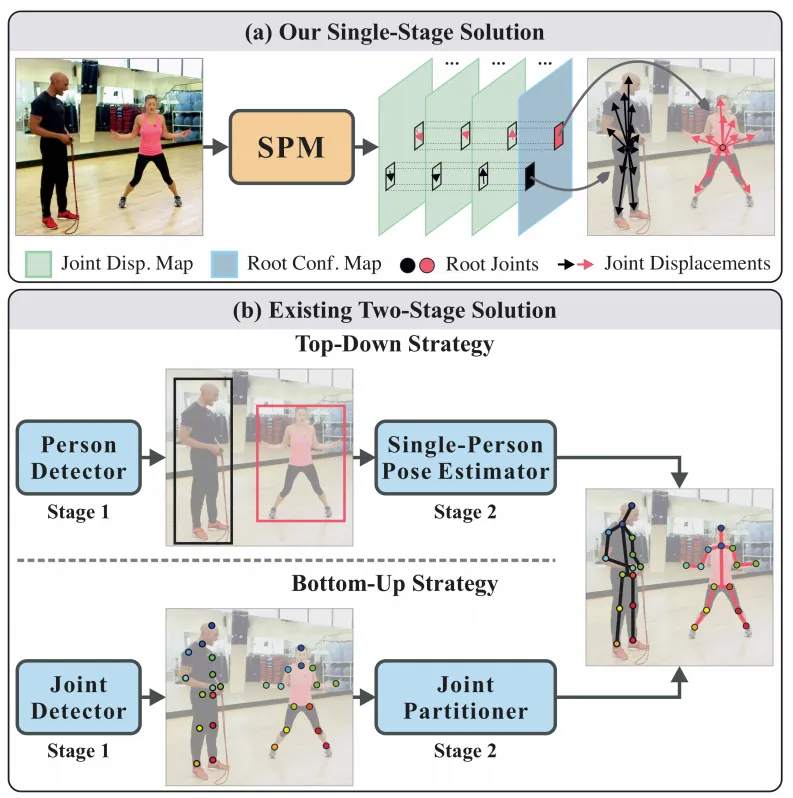
\includegraphics[width=11cm]{figure/ch2_fig_topvsbottom.png}
     \caption[辨識關節點位置的方法 ~\cite{nie2019single}]{辨識關節點位置的方法 ~\cite{nie2019single}}
     \label{ch2_fig_topvsbottom}
\end{figure}

經過影像辨識的圖像的輸出資料為熱圖 (heatmap),熱圖的概念為將一張影像分割成多個網格,每個網格內的數值代表該網格內的像素點為某個關節點的機率,將其可視化後如圖~\ref{ch2_fig_heatmap} 所示,
由左至右分別為左肩膀、左手肘、左手腕、右肩膀的熱圖,可發現對應關節點的位置會有紅色的標記,即為經過影像辨識後,判斷該像素點為該關節點的機率最高。
有學者會進一步對熱圖進行後處理,例如 OpenPose 將熱圖與其定義的 Part Affinity Fields (PAF) 結合,進一步更準確的辨識出關節點位置,
又或者如 MultiPoseNet 將熱圖與 Pose Residual Network (PRN) 結合,
從熱圖結果中篩選出研究者有興趣的關節點位置~\cite{kocabas2018multiposenet}。
因此,要使用哪一種辨識方法,是否對輸出的熱圖進行後處理,需經過學者們仔細思索自身需求,再進行選擇。
無論選擇哪一種辨識方法,最容易被大眾應用的相機為 RGB 相機 (Red-Green-Blue camera),因此蒐集到的影像資訊缺乏受試者的深度資訊,
需再透過棋盤格方法~\cite{zhang1999flexible} 進行相機校正及三角測量計算,取得受試者的三維姿態。

\begin{figure}[!ht]
    \centering
    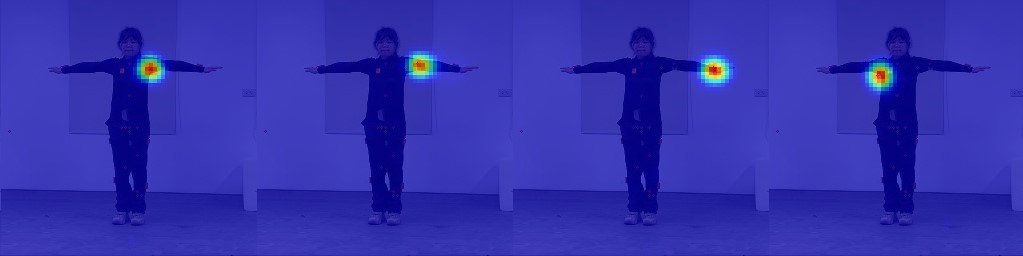
\includegraphics[width=\linewidth]{figure/ch2_fig_heatmap.jpg}
     \caption[影像辨識的輸出熱圖]{影像辨識的輸出熱圖}
     \label{ch2_fig_heatmap}
\end{figure}

使用無標記動作捕捉系統進行人體姿態重建時,誤差會受到多個因素影響,
例如輸入影像辨識模型訓練集的多樣性、受試者的姿態及服裝顏色、背景複雜程度、相機校正的準確度、相機的數量等,
因此誤差範圍較廣,例如 OpenPse 使用五台相機進行量測,其誤差約為 30 (mm)~\cite{nakano2020evaluation},
Adafuse 使用八台相機進行測量,其誤差約為 19.2 (mm)~\cite{zhang2020adafuse}。
儘管無標記動作捕捉系統的誤差無法與光標記動作捕捉系統匹敵,
但是,無標記動作捕捉系統較不受環境光限制,因此可以解決實驗場地必須設置於室內的限制,可拓展至室外進行量測,也增加了可量測的範圍及動作多樣性,
且器材架設相對容易,使用手機也可進行影像錄製,架設成本相對較低,
但其缺點為易受到遮擋而影響辨識結果,若受試者的部分關節被自身遮擋或是被場域中的其他障礙物遮擋,則無法辨識出被遮擋的關節。

\subsection{單感測器-慣性動作捕捉系統}
%  - IMU
    % - 只能量測到方向,無法量測到位置
    % - 量測時常拉長後會產生 drift 的問題
以朝向為主要量測目標的慣性動作捕捉系統,通常以可穿戴的慣性感測器 (Inertial Measurement Unit, IMU) 為量測工具,
一個測量單元包括加速規 (accelerometers)、陀螺儀 (gyroscopes) 及磁力計 (magnetometers) 三種感測器,
加速規用於測量三軸加速度,陀螺儀用於測量三軸角速度,磁力計用於測量三軸磁場強度,
透過三個感測器量得重力方向及地球磁場方向,
經由資料融合演算法推估出 IMU 當下的姿態~\cite{young2009comparison}~\cite{madgwick2011estimation}~\cite{nazarahari202140},
將 IMU 黏貼於欲量測的身體部位,例如頭部、手臂、腰部、腿等,即可量測受試者該部位的姿態。
現今最常被使用於量測人體姿態的 IMU 設備為 Movella Xsens MVN ~\cite{roetenberg2009xsens}~\cite{paulich2018xsens},
其使用無線傳輸技術傳遞量測資料,並可透過其提供的軟體進行各感測器間的時間同步與空間校正,
進而基於骨骼結構模型重建人體姿態~\cite{mcgrath2020body}~\cite{DIP:SIGGRAPHAsia:2018},如圖~\ref{ch2_fig_IMU_pose_estimate}所示,可看到受試者右邊有一個與受試者動作相同的人體模型,即為人體姿態的重建結果,
更有學者進一步使用 IMU 的量測結果計算反向跳躍能力及骶骨運動學,以評估受試者的運動表現~\cite{mcginnis2016quantifying}~\cite{miranda2022accuracy},
或是使用 IMU 進行步態分析,用於評估步態障礙患者的康復情況~\cite{wang2020imu}~\cite{uchitomi2022three},如圖~\ref{ch2_fig_IMU_gait_estimate} 所示,可經由安裝於受試者小腿的 IMU 量測數據,推估受試者的步態軌跡。

透過微機電系統 (micro-electromechanical systems, MEMS) 設計的 IMU,
其功率消耗低、體積小、重量輕、攜帶方便,因此可量測場域廣泛,不受空間限制,可以作為日常配戴的裝置,時刻監測受試者的姿態;
且其可克服在無標記動作捕捉系統中的遮擋問題,及運動速度過快產生的影像動態模糊問題。
但是,IMU 僅可量測方向,無法量測位置,且隨著量測時間拉長,
將加速度進行積分後會產生嚴重的飄移問題 (drift),從而無法計算位置資訊;
且每次測量皆需校正每一感測器與其黏貼的身體部位的相對位置及相對方向,以確保量測結果的準確性,
在量測過程中,IMU 可能會因為肌肉出力與放鬆而有相對位置的變化,
進而影響量測結果的準確性~\cite{fiorentino2017soft}~\cite{stagni2005quantification}。
慣性動作捕捉系統使用 IMU 及運動學模型、運動學限制等資訊後,可重建受試者的姿態,其整體平均位置估計誤差約為 35 (mm)~\cite{s17061257}。

\begin{figure}[!ht]
    \centering
    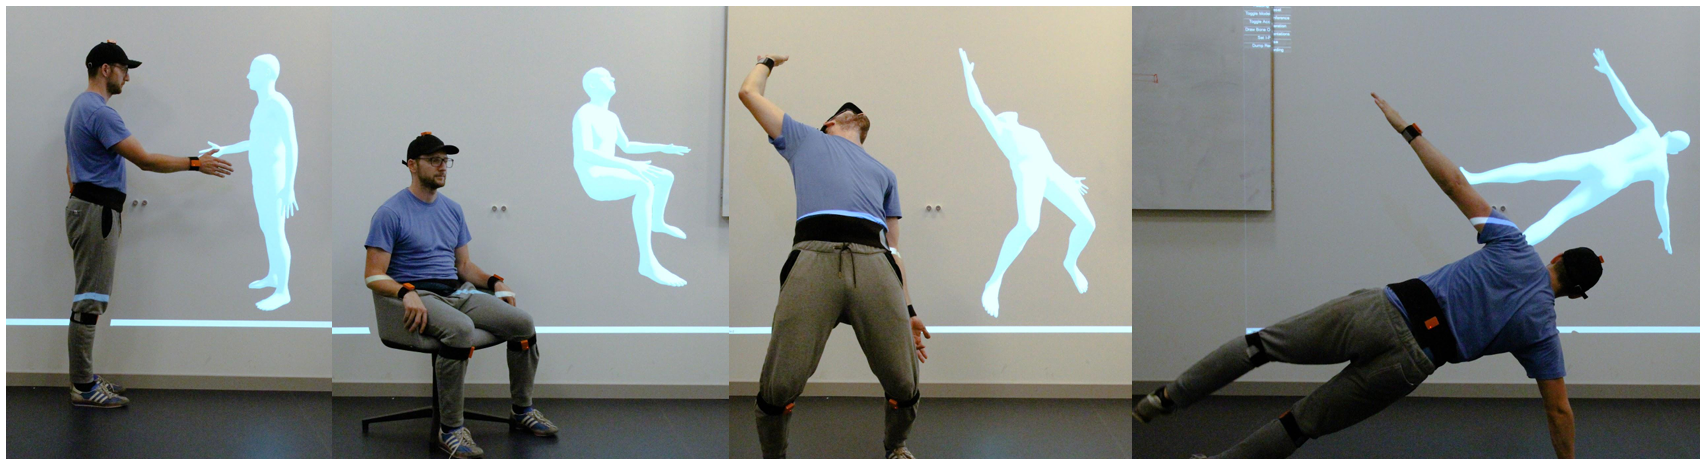
\includegraphics[width=\linewidth]{figure/ch2_fig_IMU_pose_estimate.png}
     \caption[使用 IMU 重建人體姿態 ~\cite{DIP:SIGGRAPHAsia:2018}]{使用 IMU 重建人體姿態 ~\cite{DIP:SIGGRAPHAsia:2018}}
     \label{ch2_fig_IMU_pose_estimate}
\end{figure}

\begin{figure}[!ht]
    \centering
    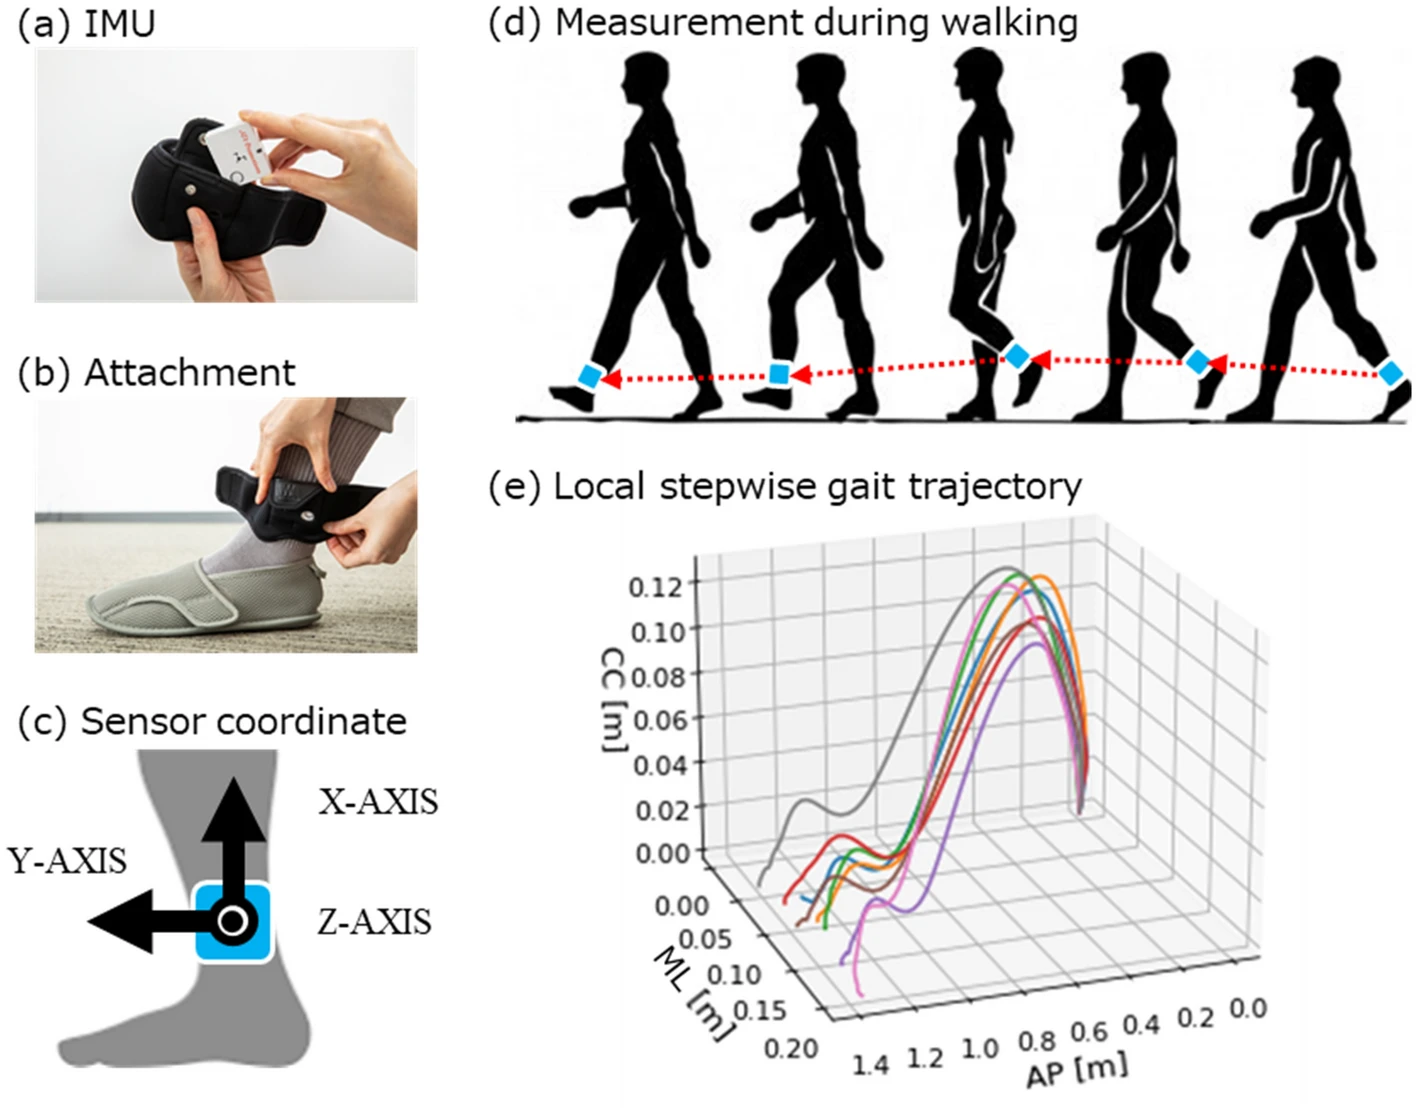
\includegraphics[width=\linewidth]{figure/ch2_fig_IMU_gait_estimate.png}
     \caption[使用 IMU 進行步態分析 ~\cite{uchitomi2022three}]{使用 IMU 進行步態分析 ~\cite{uchitomi2022three}}
     \label{ch2_fig_IMU_gait_estimate}
\end{figure}

\clearpage

\subsection{多感測器融合動作捕捉系統}
% - 相機與 IMU 融合
% - 3DPW、totalcapture、real-time full-body…、wearable fusing…
由於無標記光學動作捕捉系統會因為遮擋問題而無法辨識出被遮擋的關節,IMU 量測時長拉長會產生飄移問題,
因此,學者們開始將光學動作捕捉系統與 IMU 進行感測器融合,以彌補各自的缺點~\cite{li2023visual},
藉由 IMU 的量測資料補足光學動作捕捉系統的遮擋、移動快速產生影像動態模糊的問題,
並藉由光學動作捕捉系統不需積分的特性,解決 IMU 量測時長拉長產生飄移的問題,同時可用於計算受試者於空間中的位置資訊。

多感測器融合方法可應用於自動駕駛、智慧機器人、增強實境 (AR) 及虛擬實境 (VR) 等領域~\cite{jinyu2019survey}~\cite{zhu2023camera},
也可應用於人體動作捕捉領域,
% 人體動作捕捉範圍可包含手部、上半身、下半身、全身等不同部位,
在多感測器融合動作捕捉系統中,相機及 IMU 使用數量可有多種組合,
例如 Matthew Trumble 等人使用 4 或 8 台相機及 13 個 IMU 進行融合,建立人體全身姿態,
並發表一系列經過時間同步的多視角影片 (multi-viewpoint video, MVV) 搭配 IMU 資料集~\cite{Trumble:BMVC:2017};
或如學者 Zhe Zhang 等人使用 TotalCapture 資料集中的 4 台攝影機,及 8 個 IMU 資料融合,如圖~\ref{ch2_fig_fusing} 所示,其將結果以運動學模型的方式呈現重建的人體姿態,
並使用同資料集的 Vicon 資料驗證融合方法,誤差為 24.6 (mm) ~\cite{Zhang_2020_CVPR};
又如學者 Von Marcard 等人提出的 \textit{3D Poses in the Wild} (3DPW) ~\cite{vonMarcard2018},使用 TotalCapture 資料集驗證融合方法,誤差為 26 (mm),並發表一系列可供下載的資料集,並進一步使用一台手持相機及 6 \textasciitilde\ 17 個 IMU 融合重建人體在戶外運動的姿態。
% ,如圖~\ref{ch2_fig_3DPW} 所示,經由攝影機拍攝受試者的活動,並由 IMU 決定要重建姿態的對象,從而融合影像及 IMU 資訊,重建感興趣的受試者的姿態,因此可以發現即使有許多人存在於畫面中,也能夠重建出特定受試者的姿態。
% TODO:想加上下半身的研究
% 相機及 IMU 使用數量可有多種組合,端看學者們的需求及實驗設計。

\begin{figure}[!ht]
    \centering
    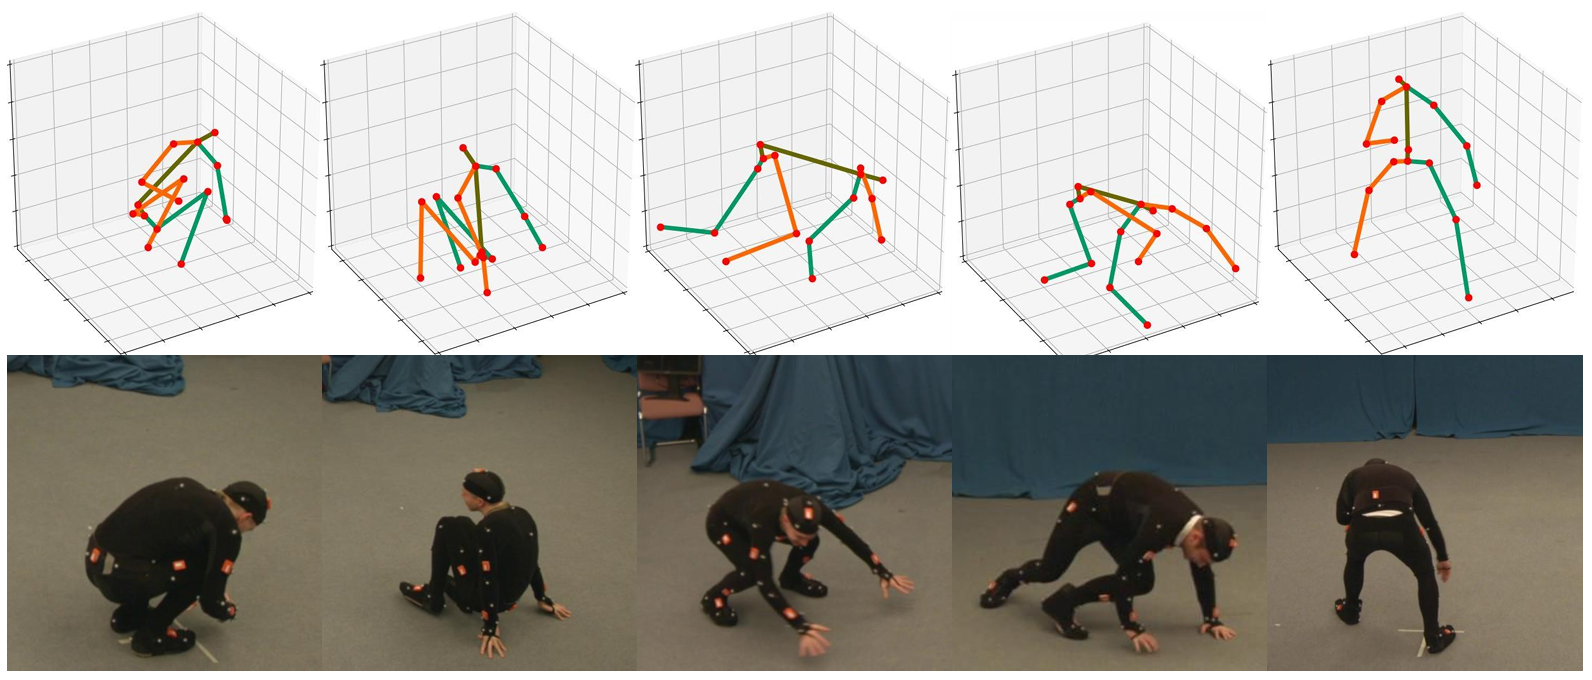
\includegraphics[width=\linewidth]{figure/ch2_fig_fusing.png}
     \caption[多感測器融合建立人體姿態~\cite{Zhang_2020_CVPR}]{多感測器融合建立人體姿態~\cite{Zhang_2020_CVPR}}
     \label{ch2_fig_fusing}
\end{figure}

% \begin{figure}[!ht]
%     \centering
%     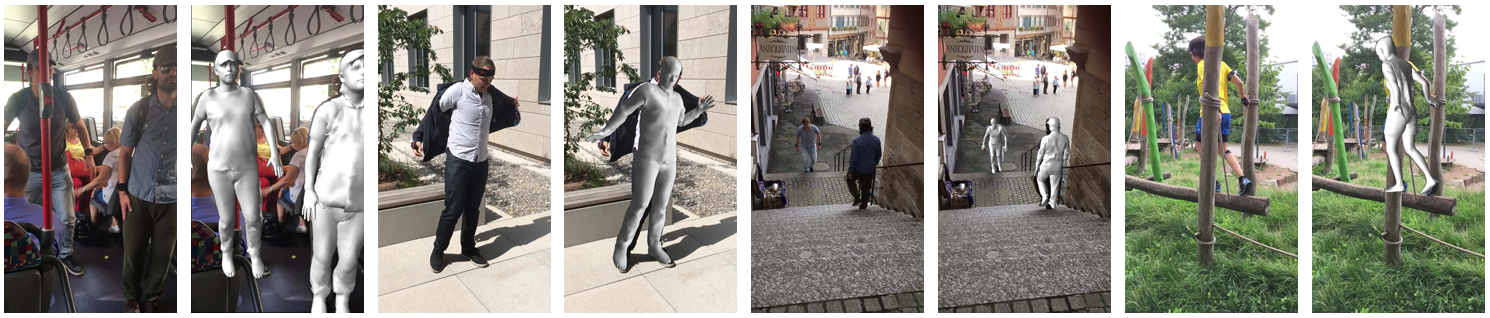
\includegraphics[width=\linewidth]{figure/ch2_fig_3DPW.png}
%      \caption[多感測器融合建立人體姿態~\cite{vonMarcard2018}]{多感測器融合建立人體姿態~\cite{vonMarcard2018}}
%      \label{ch2_fig_3DPW}
% \end{figure}

\clearpage

% ------------------------- 2.2 ------------------------- %
\section{個人化人體模型}
% 個人化骨架,還沒頭緒要寫什麼
% - 可能可以提及前人的做法,例如使用 Vicon 作為骨架,但是這樣的骨架不夠個人化,所以我要做這些事情
在人體姿態估計領域,使用動作捕捉系統過程中,通常會參考人體模型的骨架結構及物理限制,以避免估計出不符合人體結構的姿態,
而在動作捕捉系統建立人體姿態後,也常會使用人體模型 (human body model) 來描述與表示受試者的姿態,
% 因此需建立一個個人化的人體模型,
其符合受試者的骨架結構、體型及物理限制,以提高姿態估計的準確性,
如圖~\ref{ch2_fig_personal_model} 所示,
依照模型包含的資訊不同,人體模型可分為運動學模型 (Kinematic Model)、平面模型 (Planar Model)、體積模型 (Volumetric Model) 三類,
人體模型可用於描述人體結構、人體形狀及人體表面紋理等資訊~\cite{gong2016human}。

\begin{figure}[!ht]
    \centering
    \begin{minipage}{.33\textwidth}
       \centering
       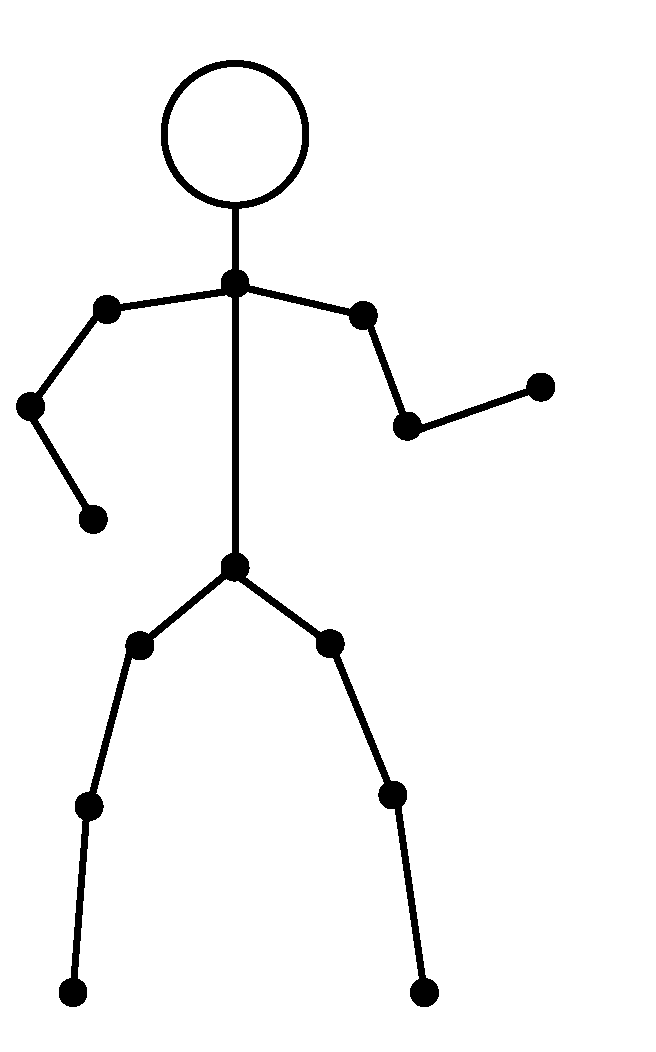
\includegraphics[width=.95\linewidth]{figure/ch2_fig_personal_kinematic_model.png}
       \caption*{(a) 運動學模型}
    \end{minipage}%
    \begin{minipage}{.33\textwidth}
       \centering
       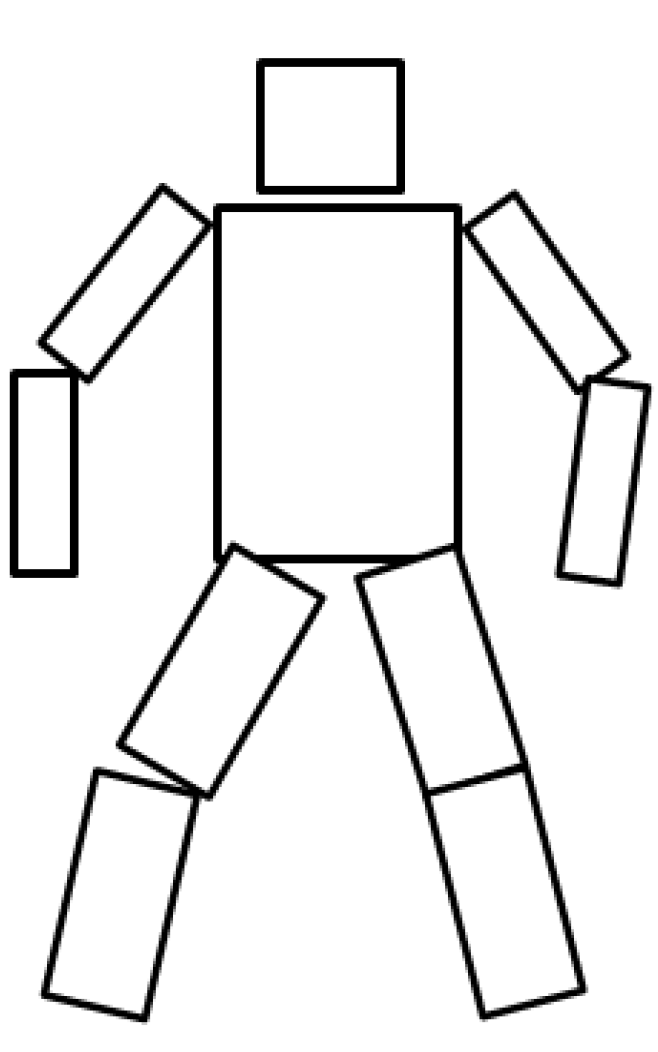
\includegraphics[width=.95\linewidth]{figure/ch2_fig_personal_volumetric_model.png}
       \caption*{(b) 平面模型}
    \end{minipage}%
    \begin{minipage}{.33\textwidth}
      \centering
      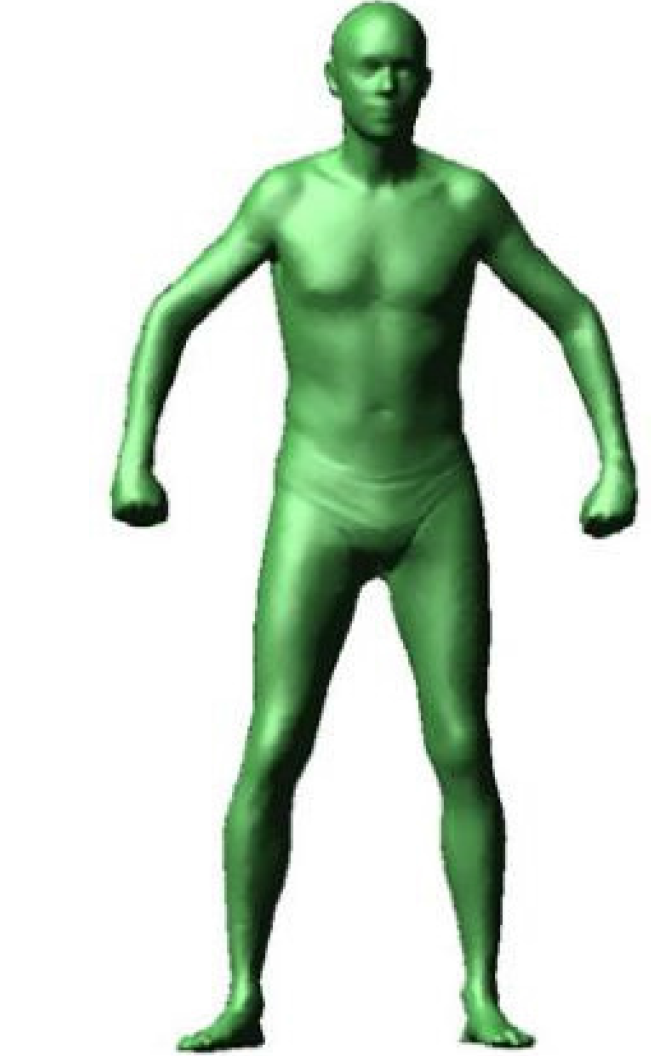
\includegraphics[width=.95\linewidth]{figure/ch2_fig_personal_planar_model.png}
      \caption*{(c) 體積模型}
    \end{minipage}
    \captionsetup{justification=centering}
    \caption[三種人體模型~\cite{gong2016human}]{三種人體模型~\cite{gong2016human}}
    \label{ch2_fig_personal_model}
 \end{figure}

\subsection*{運動學模型}
運動學模型是最常見且最頻繁被應用的模型,可用於描述二維或三維人體姿態,
通常只考慮人體骨架結構,不考慮人體的肌肉組織,以點描述關節位置,並以 bar 連接關節,代表人體指定肢體的骨骼方向,
因此運動學模型可以淺顯易懂的方式描述人體部位間的關係,但無法描述人體的形狀及表面紋理。

運動學模型可分為兩類,一類為預定義模型 (predefined model),另一類為學習圖像結構模型 (learned graph structure model)。
預定義模型結構為基於人體解剖學與物理定義所建構,其關節點名稱、層級與父子關係皆有既定定義,
不受動作捕捉數據影響,不涉及任何機器學習過程,例如 Vicon 系統中的骨架結構。
除 Vicon 系統的骨架結構外,也有學者使用預定義模型描述人體姿態估計,例如 DeepPose ~\cite{Toshev_2014_CVPR},
或是基於預定義模型進行機器學習,以約束結果符合人體結構~\cite{wei2016convolutional}。
預定義模型具有明確的物理意義,且易於解釋,但模型結構較為簡化,因此無法捕捉複雜且具有細節的運動模式。

學習圖像結構模型則從大量的人體運動圖像數據中學習人體的結構,從而建構起人體的模型,
學習圖像結構模型的方法十分多樣,一種最為常見的模型為圖像結構模型 (Pictorial Structure Models, PSM)~\cite{johnson2010clustered},
學習圖像模型可以捕捉複雜的運動模式,具有較好的人體描述能力,且模型可從數據中學習到更多的特徵,減少人工設計的成分,
但模型結構較為複雜,且可能缺乏明確的物理意義,因此難以解釋。

\subsection*{平面模型}
平面模型則是將人體分割成多個平面,以平面描述人體的外觀及形狀,
身體各部位由與人體部位相似的矩形組成,可被用於描述二維人體姿態,
例如 Active Shape Model (ASM),其使用主成分分析方法 (principal component analysis, PCA) 取得完整的人體形狀及輪廓,
以表示人體全身姿態~\cite{freifeld2010contour}。平面模型由於組成比體積模型簡單,因此計算速度較快,
但是因為只能描述二維人體姿態,缺乏深度資訊,因此對於複雜的三維人體姿態描述能力較差。

\subsection*{體積模型}
體積模型包括人體的形狀資訊,人體部位由相似形狀的圓柱體或圓錐體描述,圓柱體或圓椎體間的接點即為關節,
或是使用數千個網格組成人體表面,形成人體體積模型,可被用於描述三維人體姿態,模型的樣貌最接近人體型態,
例如學者 Matthew Loper 等人提出的 SMPL 模型 (Skinned Multi-Person Linear model)~\cite{SMPL:2015},
SMPL 模型為一款開源的人體體積模型,由 23 個關節及 6890 個網格頂點組成,可用於描述人體的形狀及姿態,
體積模型可以描述人體的形狀及表面紋理,且具有較好的人體描述能力,但是模型結構較為複雜,且計算速度較慢。

\clearpage

% ------------------------- 2.3 ------------------------- %
\section{時間同步}
% 時間同步的重要性
感測器間皆有各自的計時器及採樣頻率,因此無論是使用同類型感測器或是融合不同類型的感測器,皆需考慮使用的資料點是否位於相同的時刻,
若資料點不在相同時刻,則需進行時間同步 (time synchronization) 的處理,以確保資料點的一致性。
最常見的時間同步方法,一為使用硬體觸發器,透過硬體觸發器同時觸發所有感測器進行採樣,確保所有感測器的資料點位於相同時刻;
二為使用預先定義的動作進行時間同步,
例如使用拍手動作,透過拍手發出的聲音進行影像間的時間同步,
再透過拍手時巨大的加速度變化進行 IMU 與影像間的時間同步~\cite{pons2012data};
或是使用垂直跳躍或跺腳等動作,透過動作開始的時間點進行影像同步,
再透過動作中的加速度變化同步 IMU 與影像的時間~\cite{destelle2014low}~\cite{Trumble:BMVC:2017};
抑是直接使用受試者的動作進行時間同步,例如直接尋找影像中受試者走路時腳與地面接觸的時間點,
在影像方面,可以直接從影像辨識到的踝關節運動進行推測,
在 IMU 方面,可透過貼於腳上的 IMU 的加速度測量值中計算出腳與地面接觸的時間點~\cite{kaichi2020resolving};
也可使用 LED 燈及遠紅外光 LED 燈進行時間同步,透過 LED 燈的閃爍進行影像間的時間同步~\cite{nakano2020evaluation}~\cite{needham2021accuracy}。
% 上述之時間同步方法,皆有對應適合的感測器,因此在選擇時間同步方法時,需依照研究需求進行選擇。

% ------------------------- 2.4 ------------------------- %
\section{感測器融合演算法}
% 感測器融合演算法
使用多種不同感測器量測人體姿態,其資料間可能存在不同的誤差或雜訊,因此需進行感測器融合 (sensor fusion) 處理,
感測器融合方法可依照融合層級分類為原始資料層級融合 (Raw Data-Level Fusion)、特徵層級融合 (Feature-Level Fusion)、
決策層級融合 (Decision-Level Fusion) ~\cite{majumder2020vision};
也可依照融合演算法分類為直接融合方法 (Deterministic Method)、濾波融合方法 (Filter-Based Methods)、
最佳化融合方法 (Optimization-Based Methods)、機器學習融合方法 (Learning-Based Methods) ~\cite{li2023visual}。

% TODO:猶豫要不要把層級融合的圖放上去,如果要放應該是放層級融合那篇的 fig3

\subsection*{直接融合方法}
% 直接融合方法 (Deterministic Method) 使用簡單的邏輯計算或是加權平均計算,不涉及複雜的模型或算法,
% 將多個感測器的資料直接合併得到最終的姿態估計。
直接融合方法 (Deterministic Method) 屬於決策層級融合,
在執行直接融合前,無標記光學動作捕捉系統及慣性動作捕捉系統皆已完成數據蒐集、特徵提取、姿態估計,
直接融合方法僅將兩者的結果進一步進行邏輯計算或是加權平均,得到最終的姿態估計,
不涉及複雜的模型或算法,也不涉及原始數據的修正及是否提取特定特徵的判斷。
例如學者 Masataka Yamamoto 等人為了提高人體踝關節角度的估計準確度,
將慣性動作捕捉系統的加速度及角加速度數據與無光標記動作捕捉系統數據使用互補濾波器進行融合~\cite{yamamoto2022verification};
又如學者 Grzegorz Glonek 等人,分別計算出兩種捕捉系統的軸關節角度,
並依無光標記動作捕捉系統的關節狀態是否可見,決定其結果是否可靠,從而決定兩者的融合權重~\cite{s17122857}。

直接融合方法的優點為計算簡單直接,不需要複雜的模型及冗長的計算,但是每一種量測方法都存在誤差及雜訊,
直接融合方法沒有對誤差及雜訊進行處理,將這些誤差及雜訊也一併進行融合,因此可能會導致融合結果不夠準確。

\subsection*{濾波融合方法}
在需要即時處理多模態且帶有雜訊的感測器數據時,濾波融合方法 (Filter-Based Methods) 是一種常見的原始資料層級融合方法,
在執行濾波融合時,輸入通常是 IMU 的原始加速度、角速度及影像的特徵點座標,融合過程中直接對原始資料進行濾波處理,估計人體姿態。
較常被使用的濾波器包括卡爾曼濾波器 (Kalman Filter)、擴展卡爾曼濾波器 (Extended Kalman Filter)、無跡卡爾曼濾波器 (Unscented Kalman Filter),
例如學者 S. M. Orozco-Soto 等人,使用卡爾曼濾波器融合 IMU 資訊及影像資訊,估計受試者的上肢關節角度~\cite{orozco2019development},
又如學者 Randa Mallat 等人,使用擴展卡爾曼濾波器融合 IMU 資訊及影像資訊,估計受試者的上肢關節角度,
藉此評估人類上肢康復過程中的活動能力~\cite{mallat2020upper}。

濾波融合方法可以對原始資料進行濾波處理,去除雜訊及誤差,提高融合結果的準確性,且計算複雜度低,可以及時估計人體姿態,
但是濾波融合方法需要對濾波器進行參數調整,需要有準確的模型及參數,否則模型誤差可能會影響融合結果的準確性。

\subsection*{最佳化融合方法}
% 最佳化融合方法 (Optimization-Based Methods) 取決於輸入資訊決定其為原始資料融合、特徵層融合或是決策層融合,
在執行最佳化融合方法 (Optimization-Based Methods) 前,無標記光學動作捕捉系統及慣性動作捕捉系統皆已完成數據蒐集、特徵提取,
透過建立最佳化模型,將兩者的特徵透過目標函數、限制條件進行最佳化,得到最終的姿態估計。
如學者 Charles Malleson 等人,透過建立包含朝向項、位置項、加速度項等項次的目標函數,
並使用 Ceres non-linear least-squares solver 計算目標函數的最佳解,從而估計人體全身姿態~\cite{malleson2017real},
又如學者 Ahmed Ahmed 等人,使用批次最小平方法 (batch least-squares algorithm, BLS) 進行最佳化,
融合兩個黏貼於雙腳的 IMU 及頭戴式 IMU 相機,並使用不同行走狀態對應的運動約束,
以估計受試者頭部與腳部的姿勢,從而估計受試者的步態~\cite{ahmed2018visual}。

最佳化融合方法透過建立目標函數及多項限制條件的方式,將 IMU 與影像的特徵進行最佳化融合,
且可以根據不同的應用場景及需求,建立不同的目標函數及限制條件,提高融合結果的準確性;
但最佳化求解過程需要較長的計算時間及大量的計算資源,且有一些最佳化演算法可能會陷入局部最佳解的誤區,而無法找到全局最佳解。

\subsection*{機器學習融合方法}
機器學習融合方法 (Learning-Based Methods) 透過機器學習的方式,
從人工標註的數據學習將 IMU 與影像的相關資訊進行融合,並建立模型,從而估計人體姿態。
例如學者 Matthew Trumble 等人,使用長短期記憶網路 (Long Short-Term Memory, LSTM) 處理關節位置估計值,
並與 IMU 相關資訊融合,得到最終人體全身估計姿態~\cite{Trumble:BMVC:2017}。
% 又如學者 Young-Woon Cha 等人,使用深度學習方法,將 IMU 與影像的特徵進行融合,
% TODO:另一個例子有空再回來寫好了,現在有點寫不下去QQ

機器學習融合方法有強大的學習能力,可以自動從原始數據開始進行特徵提取及融合,無需人工進行資料前處理或後處理,
並且可以根據不同的應用場景及需求,建立不同的模型,靈活性較高;
但是在訓練過程中,需要大量的人工標註資料,人工標註資料的準確性將直接影響模型的準確性,
同時,訓練模型需要大量的訓練參數,因此計算成本高,
且模型的解釋性較差,難以解釋模型的輸出結果。

% ------------------------- 2.5 ------------------------- %
\section{小結}
% 章節回顧;
本章節介紹現今最常被應用的人體姿態量測、估計與重建技術,包含光標記動作捕捉系統、無標記動作捕捉系統、慣性感測器動作捕捉系統及多感測器融合動作捕捉系統。透過這些系統量化人體姿態後,可計算關節角度、肢段長度、身體部位的朝向及關節位置等資訊,並應用於運動分析、醫學研究、娛樂產業等領域。因此,系統的易用性與機動程度,以及估計結果的正確性及精度,皆為重要的議題。此外,本章節也介紹了人體模型的建立,包含運動學模型、平面模型及體積模型,這些模型可用於描述人體結構、人體形狀及人體表面紋理等資訊,並應用於人體姿態估計領域。最後,本章節介紹了感測器融合演算法,包含直接融合方法、濾波融合方法、最佳化融合方法及機器學習融合方法,這些方法可用於將多種不同感測器的資料進行融合,以提高人體姿態估計的正確性及精度。

% 重述困境;誤差是否可接受
然而,目前的人體姿態估計技術仍存在一些問題。例如,有些方法使用 Vicon 系統提供的三維人體模型作為將 IMU 朝向資訊轉換為位置資訊的媒介,因此仍未達到不借助 Vicon 系統,即能完成人體姿態量測、估計與重建的目標。且在眾多學者提供的資料集中,學者們皆已完成時間同步與空間校正等事前準備工作,因此即使受試者將影像及慣性感測器資料準備齊全,仍無法直接輸入感測器融合程式進行人體姿態重建。此外,現今存在的感測器融合實驗皆使用多台設備進行量測,因此在實驗過程中,受試者需穿戴多個感測器外,還需架設多台相機,不僅增加了實驗的複雜度,也增加了受試者的負擔,因此,如何在減少實驗設備的同時,又不顯著增加誤差,是一個值得探討的議題。

% 論文重點;章節安排
綜上所述,本論文著重於解決上述問題,改善先前學者們提出的方法,不借助 Vicon 系統完成人體姿態量測、估計與重建,並探討減少實驗設備對誤差的影響,是否在應用團隊可接受的範圍內。本論文將在第三章介紹本研究的方法及流程,第四章介紹本研究的實驗設計及實驗結果,第五章進行討論及結論並提出未來研究方向。

\clearpage